\documentclass[letterpaper]{article}
    \usepackage{amsmath}
    \usepackage{tikz}
    \usepackage{epigraph}
    \usepackage{lipsum}
    \usepackage{glossaries}
    \usepackage{graphicx}
    \usepackage{imakeidx}
    \usepackage{hyperref}
    \graphicspath{{Images/}}
    \setcounter{tocdepth}{2}
    \makeglossaries
    \makeindex[columns=2, title=Alphabetical Index]
    \renewcommand\epigraphflush{flushright}
    \renewcommand\epigraphsize{\normalsize}
    \setlength\epigraphwidth{0.7\textwidth}

    \definecolor{titlepagecolor}{cmyk}{1,.60,0,.40}

    \DeclareFixedFont{\titlefont}{T1}{ppl}{b}{it}{0.5in}

    \makeatletter
    \def\printauthor{%
        {\large \@author}}
    \makeatother
    \author{
        Brittany Lacy \\
        Drake Lambert \\
        Jeremy LeJeune \\
        Jenna Meadors \\
        Sam Miller \\
       }

    % The following code is borrowed from:  https://tex.stackexchange.com/a/86310/10898

    \newcommand\titlepagedecoration{%
    \begin{tikzpicture}[remember picture,overlay,shorten >= -10pt]

    \coordinate (aux1) at ([yshift=-15pt]current page.north east);
    \coordinate (aux2) at ([yshift=-410pt]current page.north east);
    \coordinate (aux3) at ([xshift=-4.5cm]current page.north east);
    \coordinate (aux4) at ([yshift=-150pt]current page.north east);

    \begin{scope}[titlepagecolor!40,line width=12pt,rounded corners=12pt]
    \draw
      (aux1) -- coordinate (a)
      ++(225:5) --
      ++(-45:5.1) coordinate (b);
    \draw[shorten <= -10pt]
      (aux3) --
      (a) --
      (aux1);
    \draw[opacity=0.6,titlepagecolor,shorten <= -10pt]
      (b) --
      ++(225:2.2) --
      ++(-45:2.2);
    \end{scope}
    \draw[titlepagecolor,line width=8pt,rounded corners=8pt,shorten <= -10pt]
      (aux4) --
      ++(225:0.8) --
      ++(-45:0.8);
    \begin{scope}[titlepagecolor!70,line width=6pt,rounded corners=8pt]
    \draw[shorten <= -10pt]
      (aux2) --
      ++(225:3) coordinate[pos=0.45] (c) --
      ++(-45:3.1);
    \draw
      (aux2) --
      (c) --
      ++(135:2.5) --
      ++(45:2.5) --
      ++(-45:2.5) coordinate[pos=0.3] (d);
    \draw
      (d) -- +(45:1);
    \end{scope}
    \end{tikzpicture}%
    }

%%%%%%%%%%%%%%%%%%%%%%%%%%%%%%%%%%%%
% Glossaries

\newglossaryentry{client}
{
    name=Client,
    description={The person/entity that requests a service from the service company(users of the ticketing system}
}
\newglossaryentry{technician}
{
    name=Technician,
    description={The person/entity that works a ticket}
}
\newglossaryentry{administrator}
{
    name=Client,
    description={The person/entity that manages technicians and client relations, has the power to make tickets priority}
}
\newglossaryentry{isPriority}
{
    name=isPriority,
    description={A boolean value that sets a ticket as priority, can be set by administrators}
}

\newglossaryentry{EF}
{
    name= Entity Framework,
    description={\href{https://docs.microsoft.com/en-us/aspnet/core/data/ef-mvc/?view=aspnetcore-2.1} A framework that allows for .net core applications to automatically create and manage entities such as an SQL-lite database }
}

\newglossaryentry{MVC}
{
  name= {Model View Controller},
  description={\href{https://docs.microsoft.com/en-us/aspnet/core/mvc/overview?view=aspnetcore-2.1} A Framework of application development that is used by the \gls{EF} in order to generate the SQL-lite database.}
}



\begin{document}
\begin{titlepage}

	\noindent
	\titlefont The Golden Ticket\par
	\epigraph{Software Requirements Document}%
	{\textit{}\\ \textsc{}}
	\null\vfill
	\vspace*{1cm}
	\noindent
	\hfill
	\begin{minipage}{0.35\linewidth}
		\begin{flushright}
			\printauthor
		\end{flushright}
	\end{minipage}
	%
	\begin{minipage}{0.02\linewidth}
		\rule{1pt}{125pt}
	\end{minipage}
	\titlepagedecoration
\end{titlepage}
\tableofcontents
\pagebreak
% This defines the expected readership of the document and describes its version history, including the rationale for the creation of a new version and a summary of the changes made in each version.
\section{Preface}
This document is a complete rewrite of the previously submitted version in order to better fit the format required of the requirements document. This document will contain all of the information of the previous document, and will additionally contain the sections as suggested in the textbook.

assumptions:
 \begin{itemize}
   \item The \gls{client} will not have access to the ticketing interface
   \item The boolean \gls{isPriority} will allow administrators the ability to prioritize tickets
 \end{itemize}

Summary of changes:
\begin{itemize}
	\item From the first version that was submitted early this semester this document has gone from being a list of tables to a full blown document written in LaTex .
\end{itemize}

In making this document we intend to layout the master plan for a ticketing system using Microsoft's dot net core and the C\# language. This document is intended to be read by anyone intending to create this ticketing system or those intending to use it. Understanding of the C\# language will be required in order to create this ticketing system as it was originally designed. The documentation contained at \href{https://docs.microsoft.com/en-us/dotnet/core/} may be particularly helpful in understanding the code and design of this application.
\pagebreak

% This describes the need for the system. It should briefly describe the system's functions and explain how it will work with other systems. It should also describe how the system fits into the overall business or strategic objectives of the organization commissioning the software.
\section{Introduction}
The Golden Ticket is designed to be a lightweight web based ticketing system written using the c\# language. The front end of of the ticketing system will be a responsive designed website so that it is accessible on as many devices as possible. The back-end for the sight will be a micro-services implementation hosted on a debian server featuring sql-lite, the dot net core, identity server 4, lets-encrypt,the apache web server 2.0, and more. The server will feature continuous deployment, when a revision is pushed to the master branch the server will on its check (every minute) download and deploy the change and restart any changes that are needed. In this ticketing system there will be two users of the interface, technicians and admins/managers. This is added text.

\begin{enumerate}
	\item Technicians will have access to the ticket queue and assigned tickets.
	\item Admins will have access to the ticket queue, assigned tickets (if any) and the admin portal.
	\item The ticket queue will consist of all tickets that are not marked as complete. The ticket at the top of the queue will be the ticket whose due date is closest to now / farthest past due. Their will be options to filter views on tickets, such as only tickets assigned to you, only tickets at x difficulty level, etc.
	\item A \index{ticket} ticket will consist of the following items:
	      \begin{itemize}
		      \item Title
		      \item Description
		      \item Difficulty level
		      \item A boolean isPriority that can be set by administrators to bring the ticket to the top of the list.
		      \item Contact
		      \item Company/department
		      \item notes + time entries
		      \item assigned technician
		      \item due date/ time
	      \end{itemize}
	\item A \index{contact} contact will consist of the following items:
	      \begin{itemize}
		      \item Name
		      \item Phone number
		      \item Email address
		      \item Title
		      \item Company/department name
	      \end{itemize}
	\item a \index{company} company will consist of the following items:
	      \begin{itemize}
		      \item A list of contacts
		      \item A list of associated tickets
		      \item join date
	      \end{itemize}
  \item A \index{Technician} technician will consist of the following items:
        \begin{itemize}
          \item Join date
          \item experience level
          \item Email
          \item phone
          \item list of assigned tickets
        \end{itemize}
  \item An \index{administrator} administrator will consist of the following items:
        \begin{itemize}
          \item All items contained within the technician 
          \item An additional property that tags their account as an administrator
        \end{itemize}
\end{enumerate}
\pagebreak

% This defines the technical terms used in the document. You should not make assumptions about the experiences or expertise of the reader.
\section{Glossary}
\glsaddall
\printglossaries
\pagebreak

% Here, you describe the services provided for the user. The nonfunctional system requirements should also be described in this section. This description may use natural language, diagrams, or other notations that are understandable to customers. Product and process standards that must be followed should be specified.
\section{User Requirements definition}

\begin{figure}[htbp]
  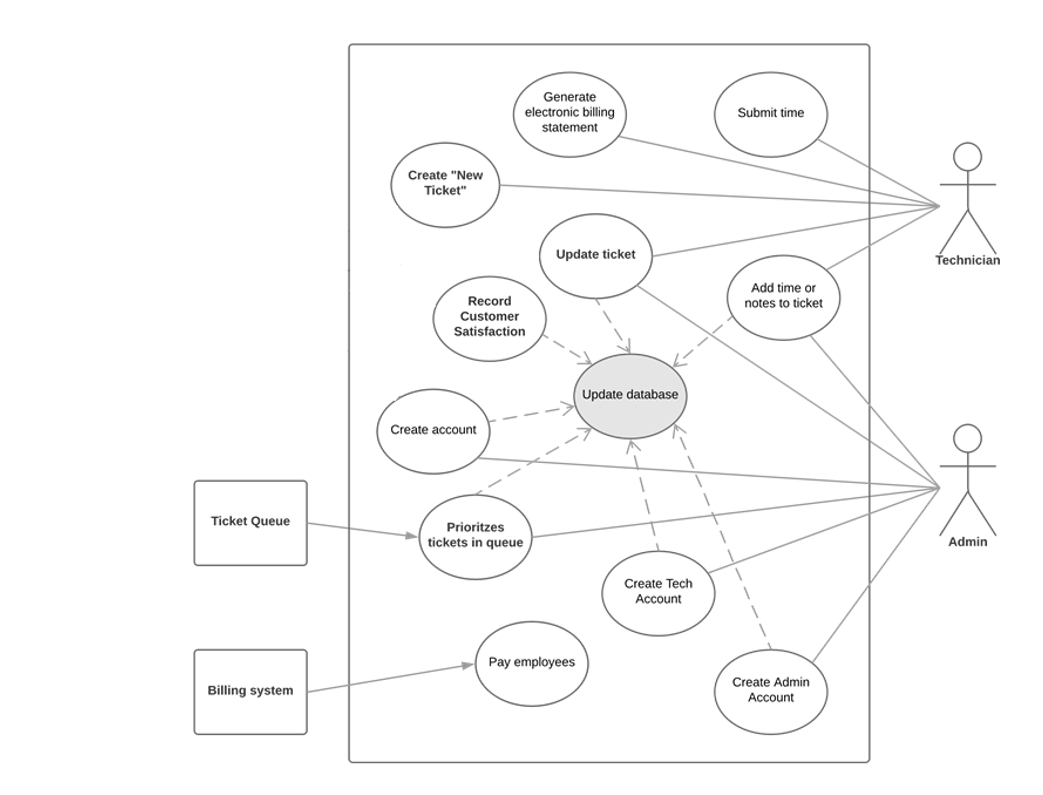
\includegraphics[]{UseCase}
  \caption{Use Case Diagram}[The above Diagram describes the use cases of the ticketing systems.]
  \centering
\end{figure}

\pagebreak


% This chapter presents a high-level overview of the anticipated system architecture, showing the distribution of functions across system modules. Architectural components that are reused should be highlighted.
\section{System Architecture}
\begin{figure}[htbp]
  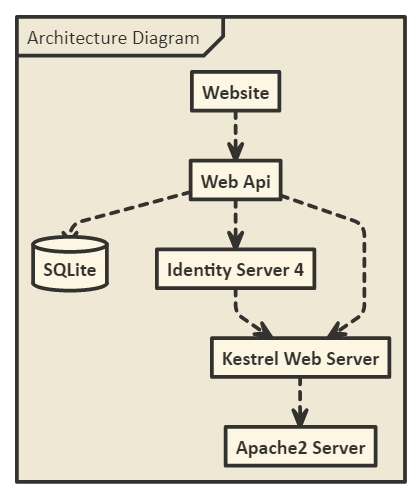
\includegraphics[scale = .5]{ArchitectureDiagram}
  \caption{Architecture Diagram}[The diagram describing the architecture of the system]
  \centering
\end{figure}
The above figure describes the main processes and applications that will be used to run this system.

\pagebreak

% This describes the functional and nonfunctional requirements in more detail. If necessary, further detail may also be added to the nonfunctional requirements. Interfaces to other systems may be defined.
\section{System Requirements Specification}

\subsection{functional Requirements}
\begin{figure}[htbp]
  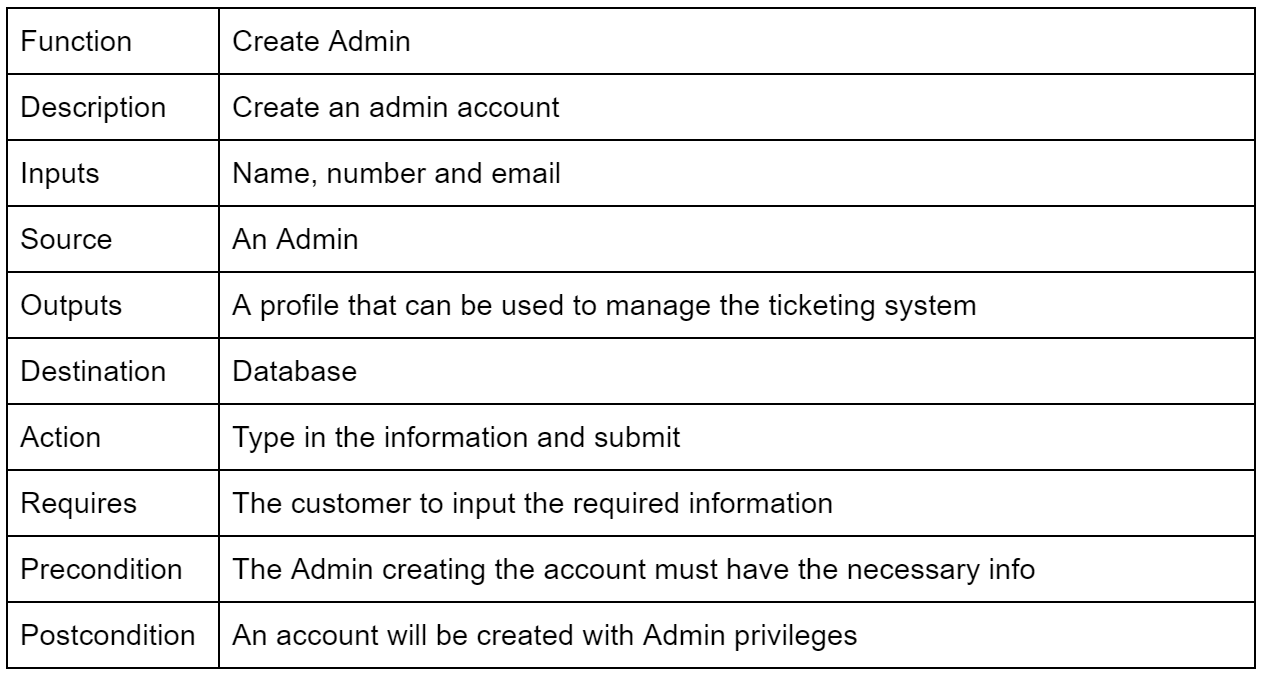
\includegraphics[scale = .5]{CreateAdmin}
  \caption{Create Admin}[The above table describes the requirements of implementing the process of creating an administrator account.]
  \centering
\end{figure}

\begin{figure}[htbp]
  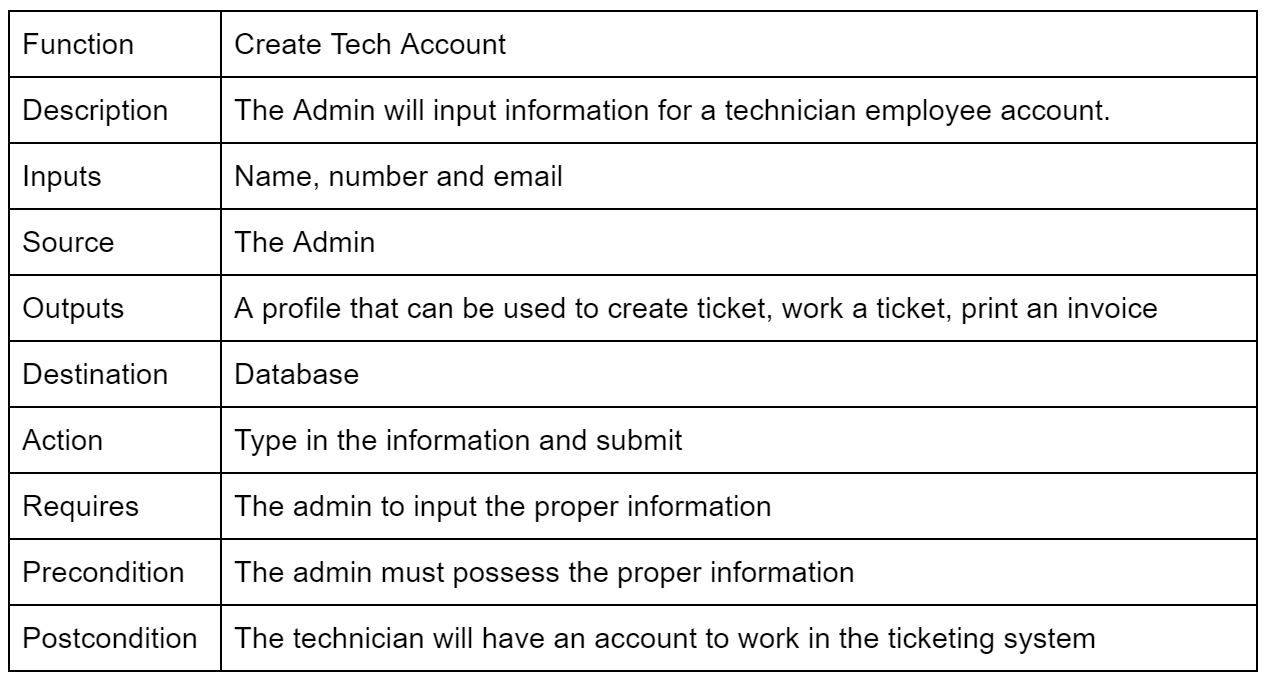
\includegraphics[scale = .5]{CreateTech}
  \caption{Create Technician}[The above table describes the requirements of implementing the process of creating a technician account.]
  \centering
\end{figure}

\begin{figure}[htbp]
  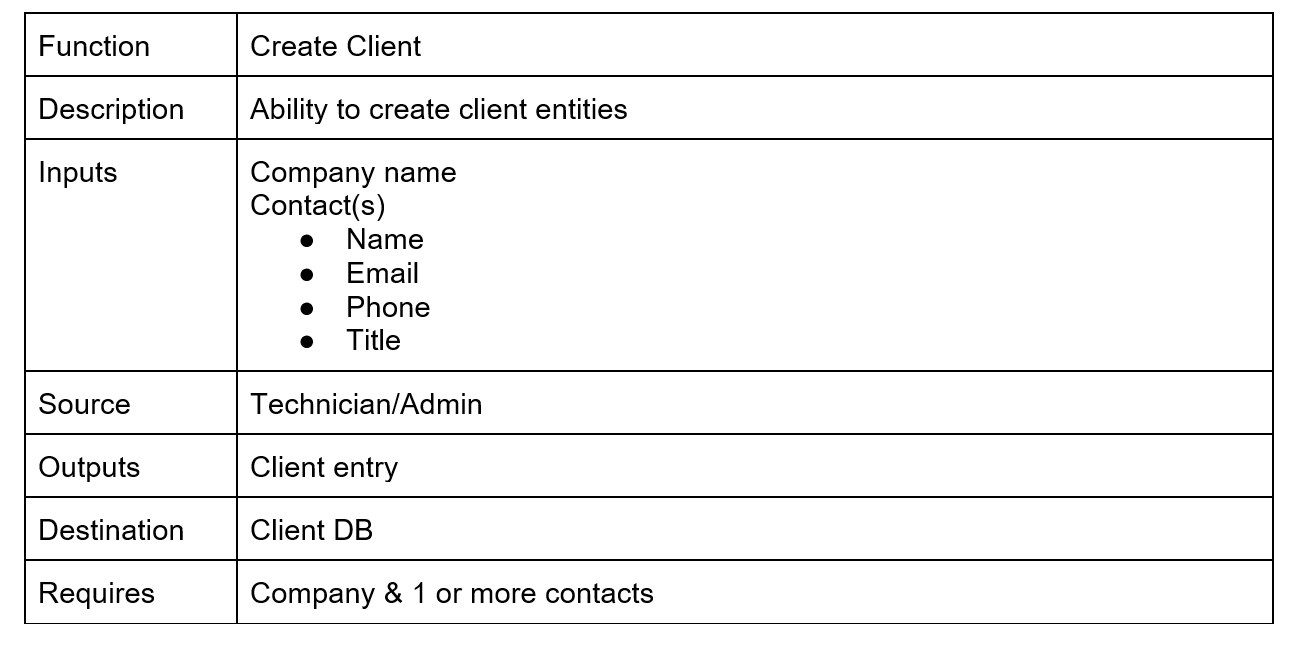
\includegraphics[scale = .5]{CreateClient}
  \caption{Architecture Diagram}[The above table describes the requirements of implementing the process of creating a client entry.]
  \centering
\end{figure}

\begin{figure}[htbp]
  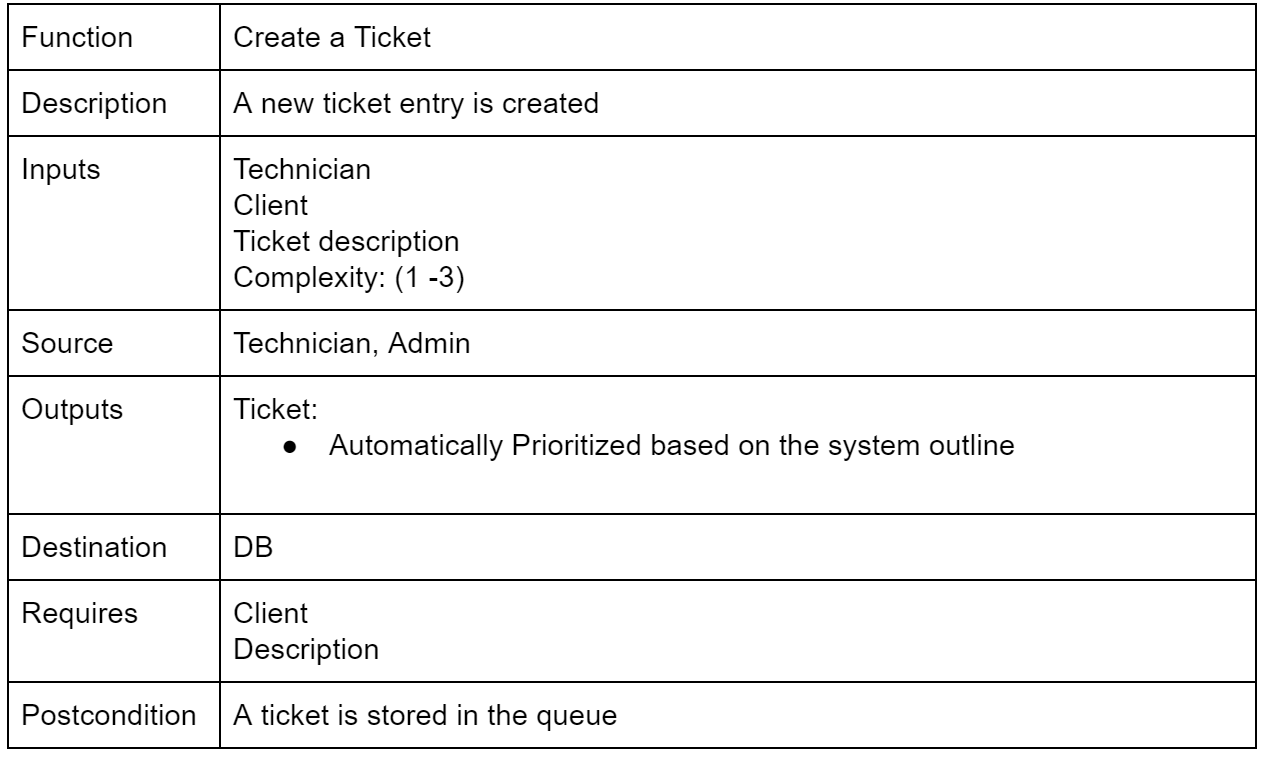
\includegraphics[scale = .5]{MakeTicket}
  \caption{Create Ticket}[The above table describes the requirements of implementing the process of creating a ticket.]
  \centering
\end{figure}


\begin{figure}[htbp]
  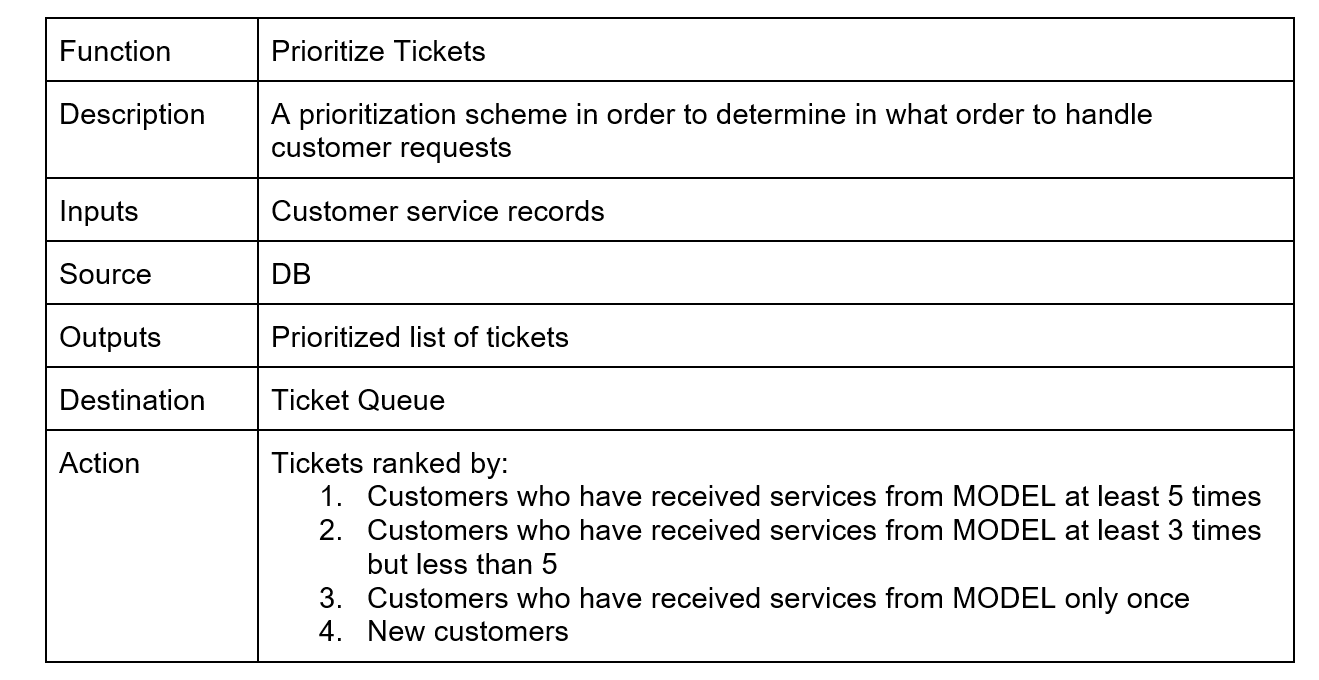
\includegraphics[scale = .5]{PrioTicket}
  \caption{Prioritize Tickets}[The above table describes the requirements of implementing the process of having the ticket queue automatically prioritized based on the number of times that a client has been served and prioritization by administrators.]
  \centering
\end{figure}

\begin{figure}[htbp]
  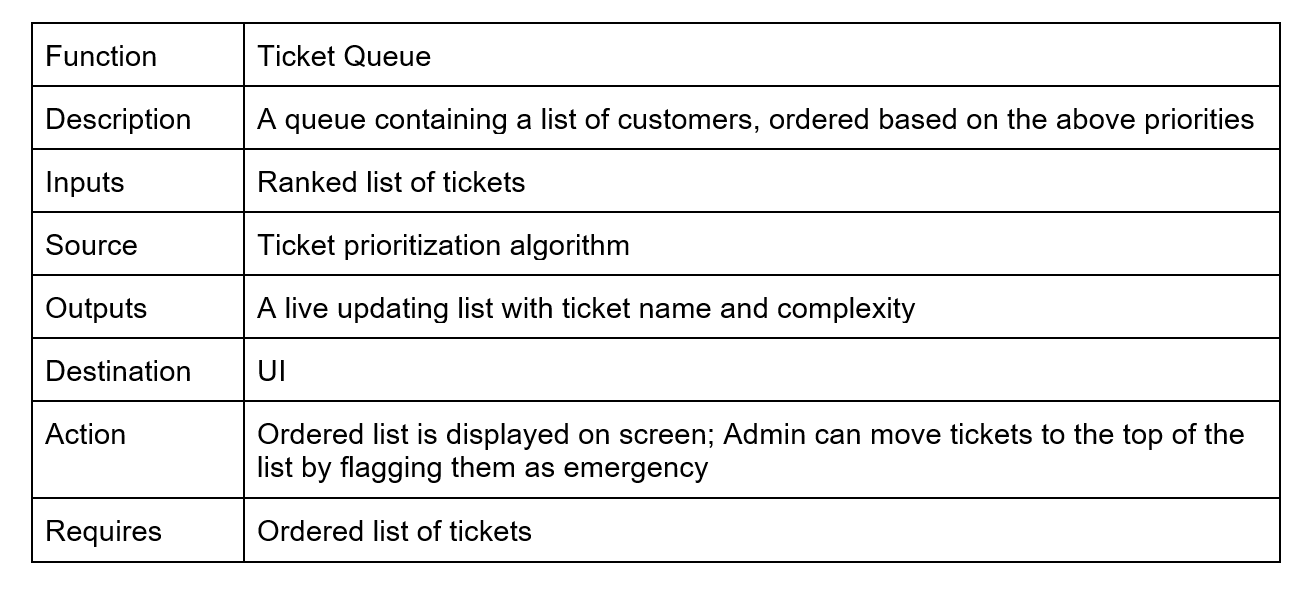
\includegraphics[scale = .5]{TicketQueue}
  \caption{Ticket Queue}[The above table describes the requirements of implementing the ticket queue.]
  \centering
\end{figure}

\begin{figure}[htbp]
  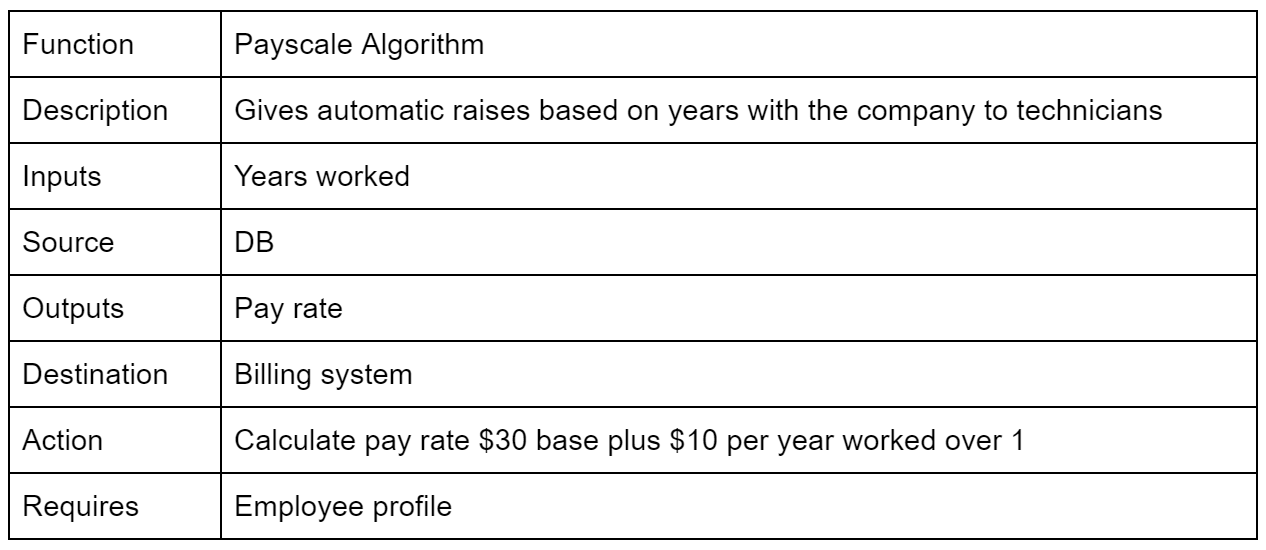
\includegraphics[scale = .5]{PayscaleAlg}
  \caption{Pay-scale Algorithm}[The above table describes the requirements of implementing the process of automatically scaling the billable rate for the technician based on the number of years of service that they have with the company.]
  \centering
\end{figure}

\begin{figure}[htbp]
  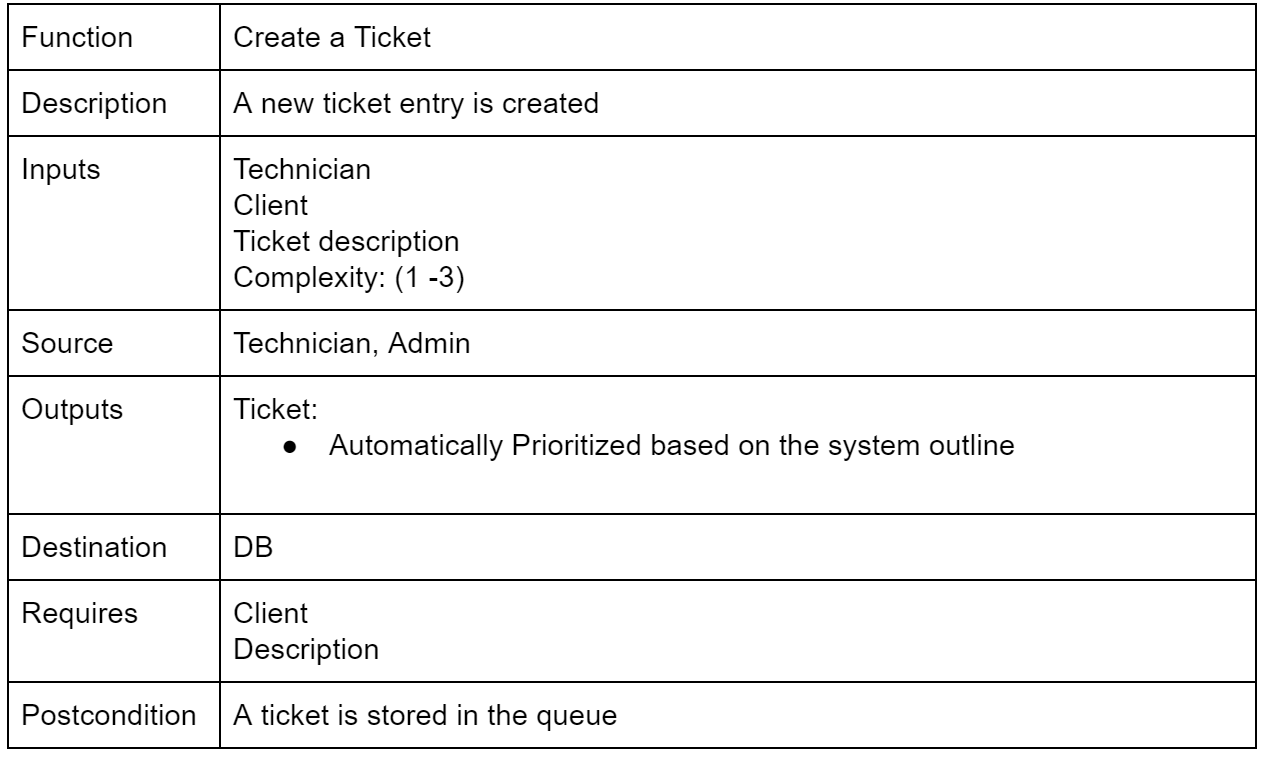
\includegraphics[scale = .5]{MakeTicket}
  \caption{Create Ticket}[The above table describes the requirements of implementing the process of creating a ticket.]
  \centering
\end{figure}

\pagebreak

\subsection{Non-functional Requirements}
\begin{itemize}
  \item  Will be developed using a platform that allows for the project to be demonstrated to the class (Web based)
  \item Our group will use UML as the primary modeling tool
  \item Our group will keep a record the date, time, length and members present for each face-to-face group meeting
  \item Our group uses GitHub as a code collaboration environment, Google Drive to share documents, Trello to stay up to date on due dates, and Discord to communicate about meeting times and share ideas. 
\end{itemize}

\pagebreak

% This chapter includes graphical system models showing the relationships between the system components and the system and its environment. Examples of possible models are object models, data-flow models, or semantic data models.
\section{System Models}
The Below model gives a broad overview of the relationships of the different components of the software system and how they interconnect and work together to provide the necessary functions of the ticketing system.
\begin{figure}[htbp]
  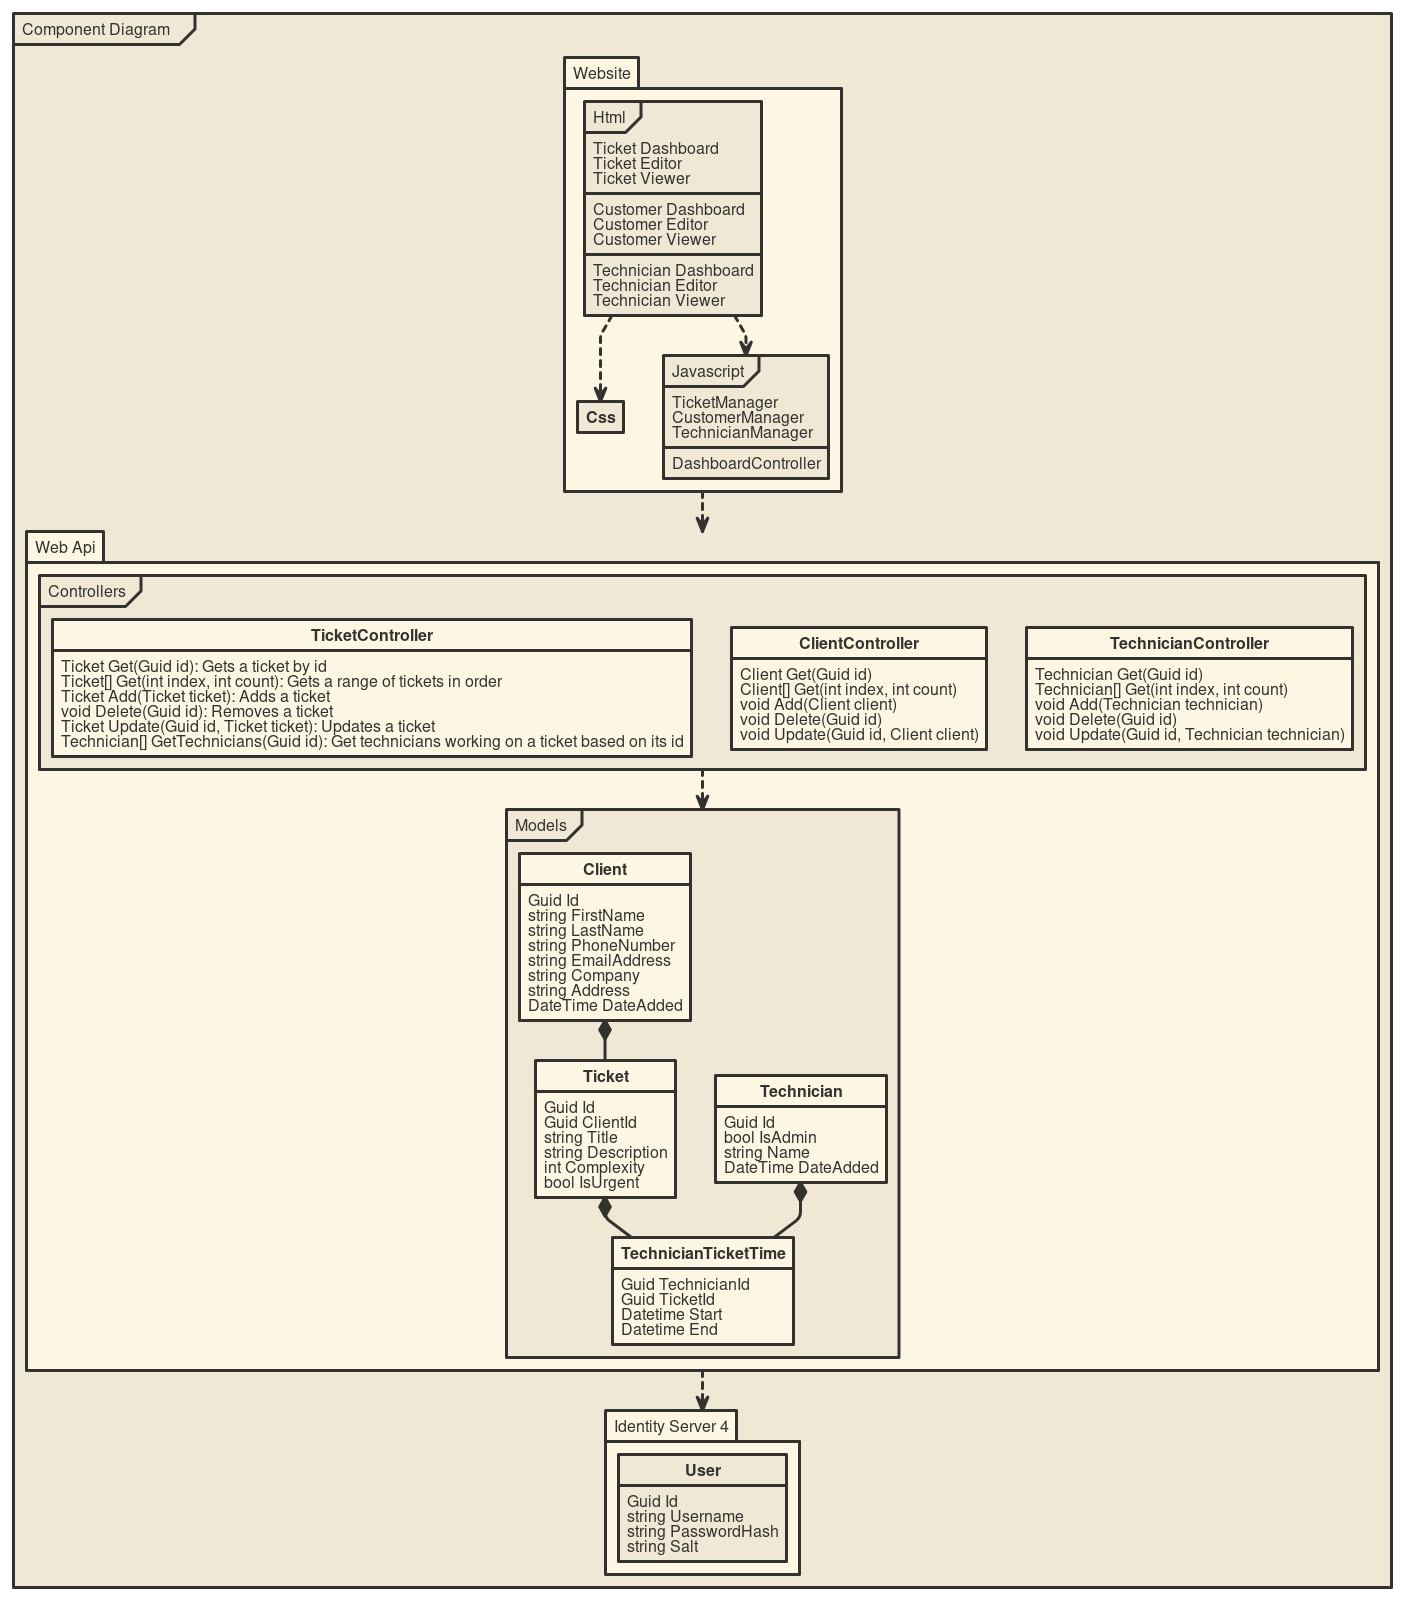
\includegraphics[scale =.3]{ComponentDiagram}
  \caption{Component Diagram}[The diagram describing the components and classes of the system]
  \centering
\end{figure}

\pagebreak

% This describes the fundamental assumptions on which the system is based, and any anticipated changes due to hardware evolution, changing user needs, and so on. This section is useful for system designers as it may help them avoid design decisions that would constrain likely future changes to the system.
\section{System Evolution}
One of the biggest assumptions we are making with this system is that the end client will not access the system in any capacity. In making this choice we are making the system more secure and the ability for the technicians to speak freely (within the companies guidelines of course)


We assume that the Tickets will be input from emails or phone calls received by administrators and or technicians. 

We assume that any and all tickets will be viewable to the pool of technicians, that administrators will ensure qualified technicians take the appropriate tickets.

We assume that admins are the only ones that can create technicians and other administrators.
\pagebreak

% These provide detailed, specific information that is related to the application being developed—for example, hardware and database descriptions. Hardware requirements define the minimal and optimal configurations for the system. Database requirements define the logical organization of the data used by the system and the relationships between data.
\section{Appendices}

\subsection{\index{Software Dependencies for host}Software Dependencies for host}
  \begin{itemize}
    \item Dotnet Runtime 2.1.104
    \item Apache2 (latest)
    \item SQL-lite (latest)
    \item Any modern operating system that can run the above.
  \end{itemize}

  Apache2 will function as a reverse proxy, instead of exposing the application directly to the web. Apache2 will receive traffic on port (if port 80 it is automatically redirected to 443) 80 or 443 and then route that traffic to localhost:5000. 
  The application itself builds and manages the SQL-lite databases using the \gls{MVC} and \gls{EF} builtin frameworks.

\subsection{\index{Hardware Dependencies for host}Hardware Dependencies for host}
  \begin{itemize}
    \item A network connection
    \item A dual core+ CPU
    \item ~ 3GB of free-space on the main storage space.
  \end{itemize}

  \subsection{\index{Software Dependencies for client}Software Dependencies for client}
    \begin{itemize}
      \item A modern web browser (edge / firefox / chrome)
    \end{itemize}

    \subsection{\index{Hardware Dependencies for client}Hardware Dependencies for client}
      \begin{itemize}
        \item any device capable of running the above web browsers
      \end{itemize}

\pagebreak

% Several indexes to the document may be included. As well as a normal alphabetic index, there may be an index of diagrams, an index of functions, and so on.
\printindex
\listoffigures
\pagebreak



\end{document}
